\documentclass{DateStructure}

\SubjectName{航空客运订票系统}
\CollegeName{理学院}
\Major{信息与计算科学}
\GroupNumber{第十六组}
\StudentA{20071226}{童繁}{流程图}
\StudentB{20071227}{王瀚功}{数据}
\StudentC{20071228}{王赛豪}{文案}
\StudentD{20071229}{吴政豪}{调试}
\StudentE{20071230}{武琦}{代码}

\begin{document}
\makecover
\newpage
\thispagestyle{empty}
\tableofcontents   
\newpage
\setcounter{page}{1}  

\section{需求分析}
\begin{itemize}
\item[(1)]设计一个航空客运订票系统,实现查询航线、客票预定和办理退票等功能。
\item[(2)]航线信息包括站名、机场、航空公司、航班号、飞机号、飞行时间、乘员定额、余票量、已订票的客户名单以及等候替补的客户名单。
\item[(3)]查询航线:根据旅客提出的起飞地-目的地和起飞日期输出航班信息,并内嵌订票功能。
\item[(4)]承办订票业务:根据客户要求,若有余票,办理订票手续并输出座位号;若已满员或余票额少于订票额,则需重新询问客户要求。若需要,可登记候补。
\item[(5)]承办退票业务:根据客户的身份证号,输出所有的订票信息,客户选择退票航班,为客户办理退票手续。然后查询该航班是否有人排队候补,首先询问排在第一的客户,若所退票额能满足他的要求,则为他办理订票手续,否则依次询问剩余候补的客户。
\item[(6)]当客户订票要求不能满足时,系统可向客户提供中转航线。
\end{itemize}

\section{项目亮点}
\begin{itemize}
\item[(1)]建立了航线信息库和客户名单库两个csv文件,方便管理员调用和修改信息;
\item[(2)]建立了独立的类型库和功能库,使得项目的调用更加清晰合理;
\item[(3)]在查询功能中内嵌了订票功能,整个系统遵循现实订票的逻辑和流程;
\item[(4)]在订票时提供了中转的路线推荐;
\item[(5)]客户可以根据自己的身份证号查询自己的所有订单,并选择想退的订单;
\item[(6)]解决了客户订票时与自己所有订单的时间冲突问题。
\item[(7)]客户可以组团订票。
\end{itemize}

\section{概要设计}
利用airline.csv存储航线信息,利用client.csv存储客户信息:航线序号、姓名、身份证号、飞机舱位。每次打开系统首先读取两个文件,每次关闭系统前重新录入更新后的信息。\par
订单中转则是找出满足地点条件和日期条件的一组航班(包含两次航班,一个中转站)。当前一个航班的到达时间与下一个航班的起飞时间在同一天且间隔时间大于一小时时,则为可行方案,待用户选择后分别下单这两次航班即可。\par
时间冲突问题是客户下单时选择的航班与客户已经订票成功的航班之间有时间交集,客户不可能同时在两趟航班上乘坐,若时间不冲突,则客户可以正常下单。\par
\begin{figure}[H] 
\centering
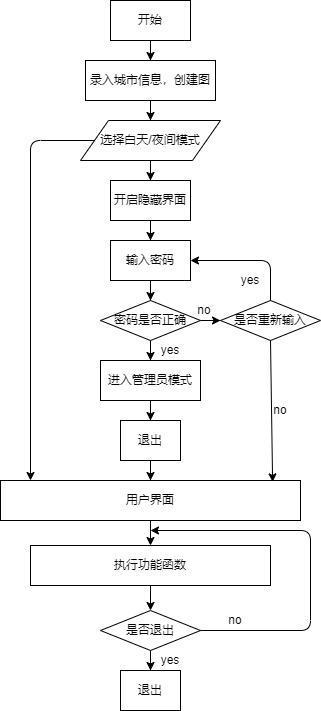
\includegraphics[width=300pt]{主函数.png}
\caption{主函数流程图}
\end{figure}

\section{详细设计}
\subsection{定义}
\lstinputlisting[language=C]{./code/definition.h}	
\subsection{类型库}
\subsubsection{List库}
\begin{figure}[H] 
\centering
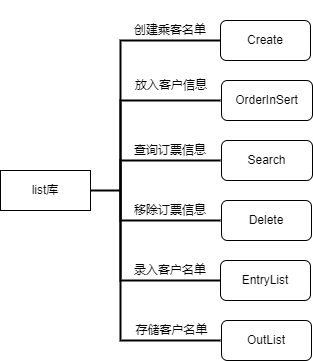
\includegraphics[width=300pt]{list.png}
\caption{List库示意图}	
\end{figure}
\lstinputlisting[language=C]{./code/list.c}
\subsubsection{Queue库}
\begin{figure}[H] 
\centering
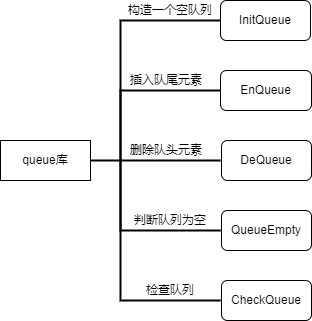
\includegraphics[width=300pt]{queue.png}
\caption{Queue库示意图}	
\end{figure}
\lstinputlisting[language=C]{./code/queue.c}
\subsubsection{Airline库}
\begin{figure}[H] 
\centering
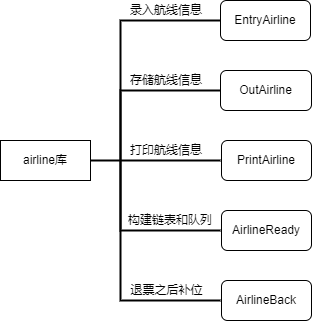
\includegraphics[width=300pt]{airline.png}
\caption{Airline库示意图}
\end{figure}
\lstinputlisting[language=C,breaklines=true]{./code/airline.c}
\subsection{功能库}
\subsubsection{查询库}
\begin{figure}[H] 
\centering
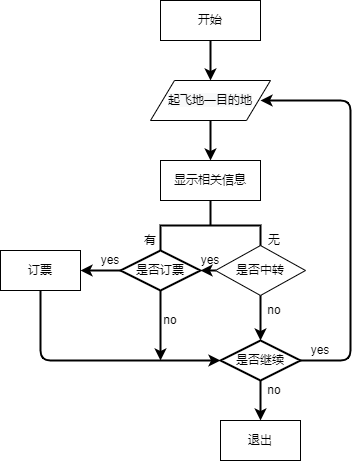
\includegraphics[width=200pt]{查询.png}
\caption{查询流程图}	
\end{figure}
\begin{figure}[H] 
\centering
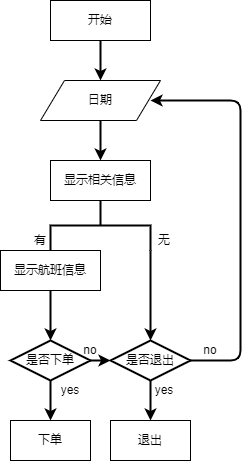
\includegraphics[width=150pt]{订票.png}
\caption{订票流程图}	
\end{figure}
\begin{figure}[H] 
\centering
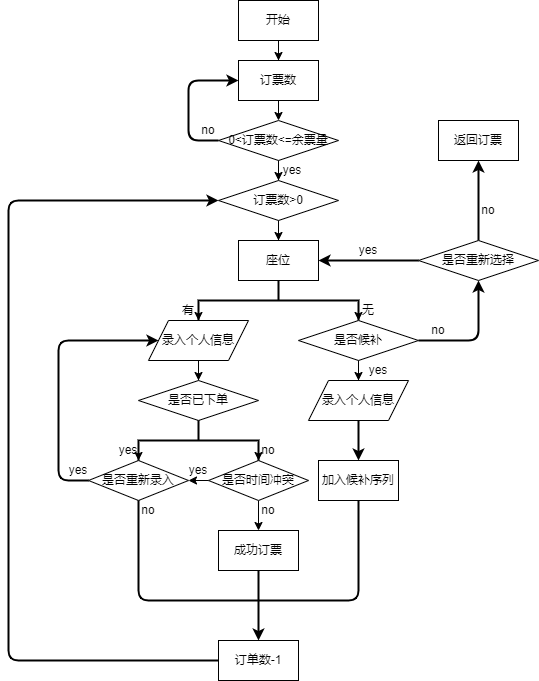
\includegraphics[width=250pt]{下单.png}
\caption{下单流程图}	
\end{figure}
\lstinputlisting[language=C]{./code/inquire.c}
\subsubsection{退票库}
\begin{figure}[H] 
\centering
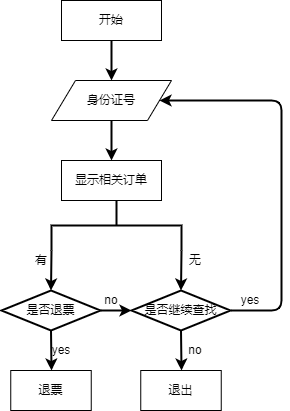
\includegraphics[width=200pt]{个人信息.png}
\caption{个人信息检索流程图}	
\end{figure}
\begin{figure}[H] 
\centering
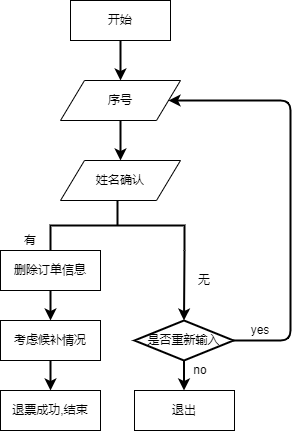
\includegraphics[width=200pt]{退票.png}
\caption{退票流程图}	
\end{figure}
\lstinputlisting[language=C]{./code/refund.c}
\section{用户手册}
\subsection{界面}
\begin{figure}[H] 
\centering
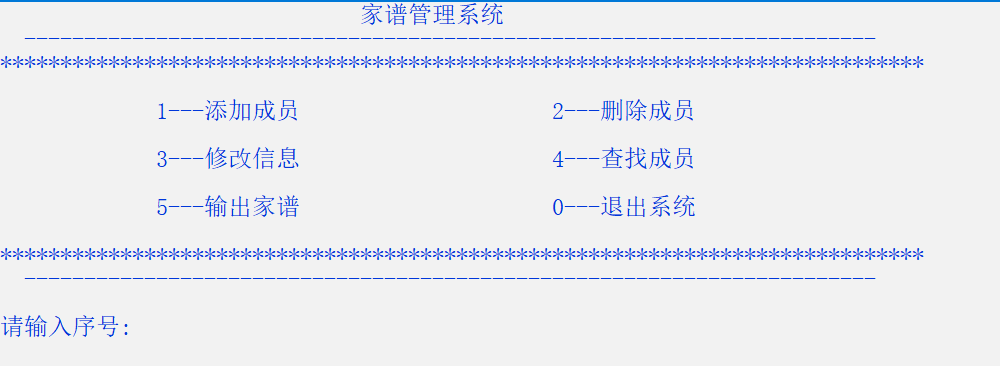
\includegraphics[width=\linewidth]{界面.png}
\caption{用户界面}
\end{figure}
\subsection{订票}
\begin{figure}[H] 
\centering
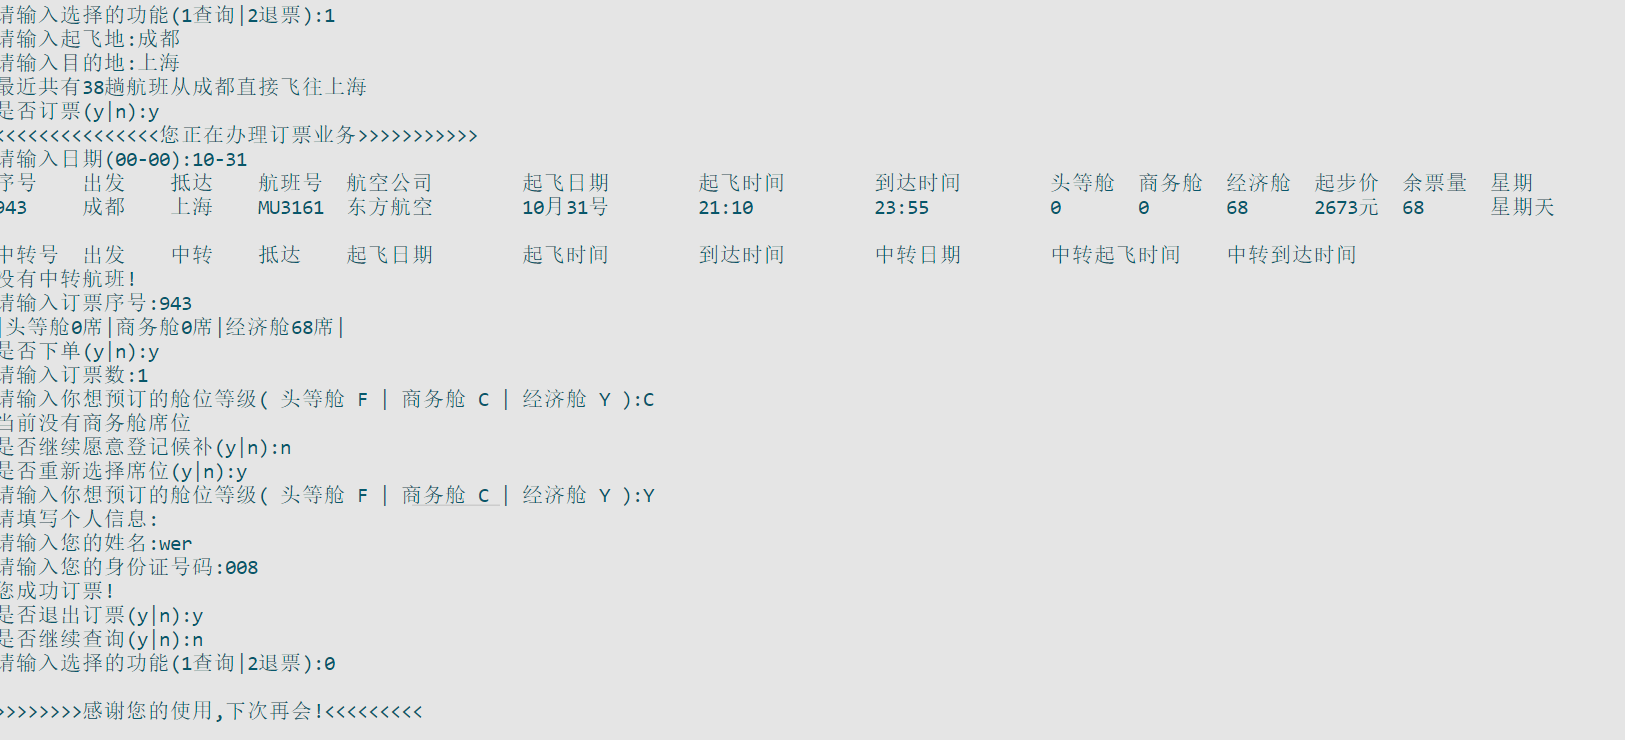
\includegraphics[width=\linewidth]{订票测试.png}
\caption{订票测试}	
\end{figure}
\subsection{候补}
\begin{figure}[H] 
\centering
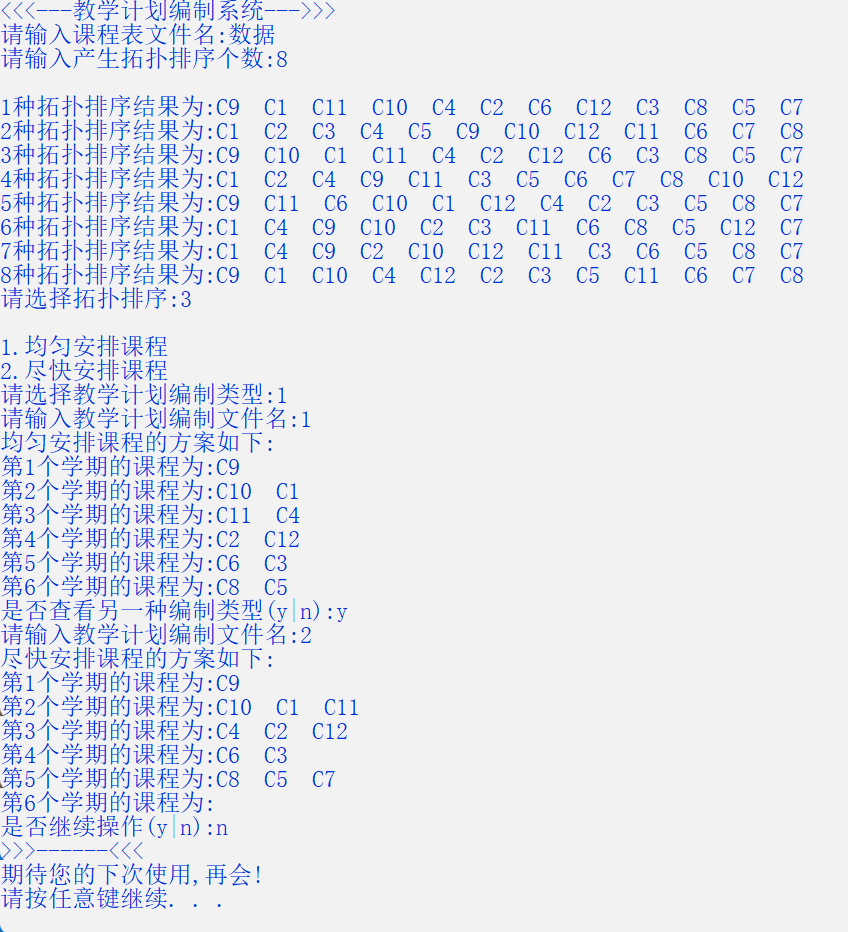
\includegraphics[width=\linewidth]{测试.png}
\caption{订票不同情况测试}	
\end{figure}
\subsection{中转}
\begin{figure}[H] 
\centering
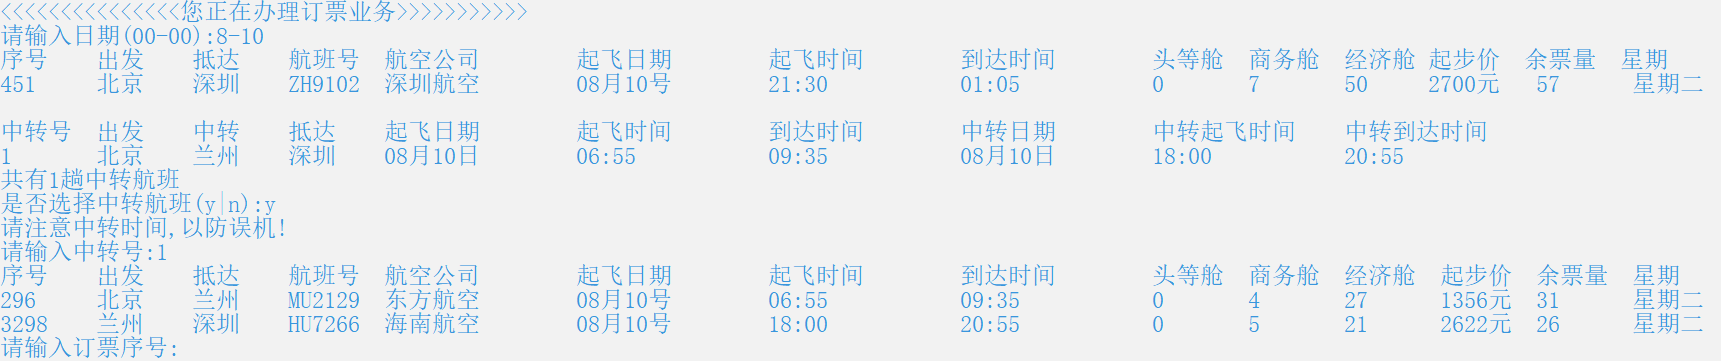
\includegraphics[width=\linewidth]{中转订票测试.png}
\caption{中转订票测试}	
\end{figure}
\subsection{时间冲突}
\begin{figure}[H] 
\centering
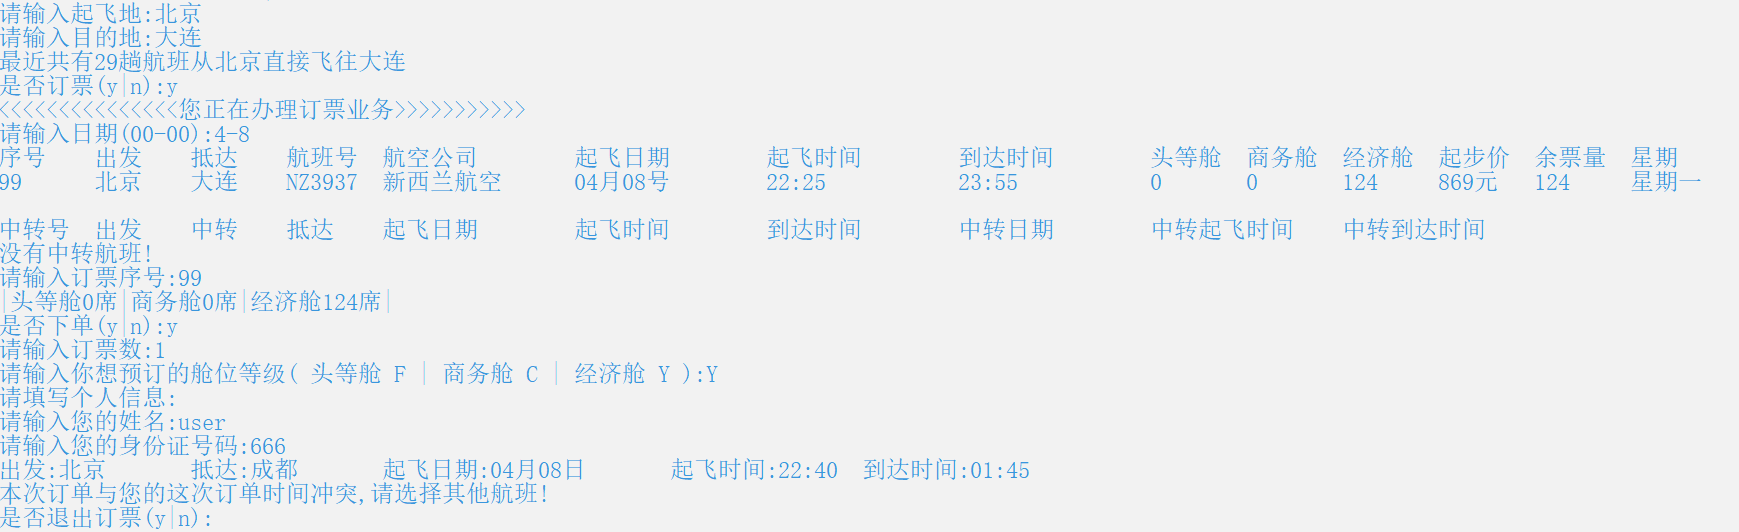
\includegraphics[width=\linewidth]{时间冲突测试.png}
\caption{时间冲突测试}	
\end{figure}
\subsection{退票}
\begin{figure}[H] 
\centering
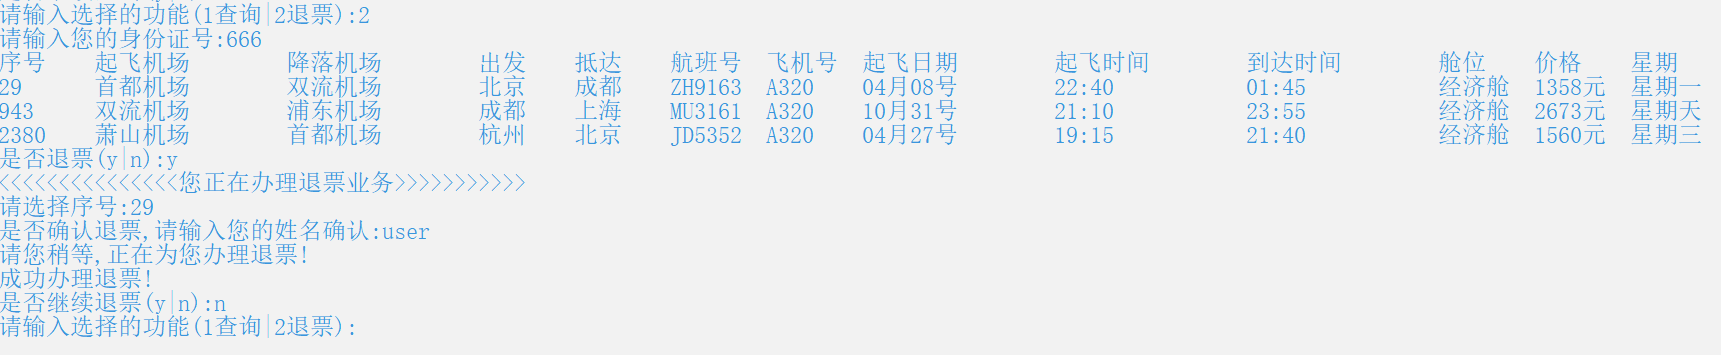
\includegraphics[width=\linewidth]{退票测试.png}
\caption{退票测试}	
\end{figure}

\section{心得体会}
这次课程设计的心得体会通过实践我们的收获如下:\par
1.在这次的航空客运订票系统的过程中,我们更深刻的了解队列的特点与用法。\par
2.在不断的修改程序bug的过程中,我们对程序运行的细节更加明了,提高了我们的查错,纠错能力。\par
3.这个课程设计考察的内容是线性表、线性链表,以及队列的综合应用,我们学会了运用伪数据库来处理数据,数据结构的理念得到了强化。\par
4.这个项目的难点不在于程序语法和算法,而是在于对整个程序架构的把握,如何摆布函数,如何理清系统的运行逻辑。\par

\newpage 
\section{附录}
\subsection{definition.h}
\lstinputlisting[language=C]{./code/definition.h}
\subsection{main.c}
\lstinputlisting[language=C]{./code/main.c}
\subsection{list.c}
\lstinputlisting[language=C]{./code/list.c}
\subsection{queue.c}
\lstinputlisting[language=C]{./code/queue.c}
\subsection{airline.c}
\lstinputlisting[language=C]{./code/airline.c}
\subsection{inquire.c}
\lstinputlisting[language=C]{./code/inquire.c}
\subsection{refund.c}
\lstinputlisting[language=C]{./code/refund.c}

\end{document}
